% ============================================================
% CASA MRes Dissertation Template
% Zhengpei (Pippin) Xu, 2025/26
% Compile: pdflatex -> biber -> pdflatex -> pdflatex
% (or just use latexmk / LaTeX Workshop default recipe)
% ============================================================

\documentclass[11pt, a4paper]{report}

% ---------- Encoding and base layout ----------
\usepackage[utf8]{inputenc}
\usepackage[T1]{fontenc}
\usepackage{lmodern}
\usepackage{geometry}
\geometry{a4paper, margin=1in}
\usepackage{setspace}
\usepackage{parskip}
\usepackage{microtype}

% ---------- Graphics, tables, maths ----------
\usepackage{graphicx}
\graphicspath{{figures/}}
\usepackage{amsmath}
\usepackage{amssymb}
\usepackage{booktabs}
\usepackage{threeparttable}
\usepackage{tabularx}
\usepackage{array}
\usepackage{longtable}
\usepackage{multirow}
\usepackage{float}
\usepackage{subcaption}
\usepackage[bottom]{footmisc}
\usepackage{enumitem}
\usepackage{makecell}
\usepackage{siunitx}

% ---------- Colours (load xcolor before hyperref) ----------
\usepackage{xcolor}

% ---------- Hyperref: teal coloured links ----------
\usepackage{hyperref}
\hypersetup{
    colorlinks=true,
    linkcolor=teal,      % footnotes, equations, cross-references
    citecolor=teal,      % bibliography citations
    urlcolor=teal        % external URLs
}

% ---------- Captions ----------
\usepackage{caption}
\captionsetup{
  font={footnotesize, color=gray, it},
  labelfont={bf, color=gray},
  justification=centering,
  labelsep=period
}

% ---------- Headers and footers ----------
\usepackage{fancyhdr}
\pagestyle{fancy}
\fancyhf{}
\lhead{\small\nouppercase{\leftmark}}   % current chapter
\cfoot{\small\thepage}
\renewcommand{\headrulewidth}{0.4pt}
% Plain style (chapter opening pages): page number only
\fancypagestyle{plain}{%
  \fancyhf{}
  \cfoot{\small\thepage}
  \renewcommand{\headrulewidth}{0pt}
}

% ---------- Chapter and section heading style ----------
\usepackage{titlesec}
\titleformat{\chapter}[hang]
  {\normalfont\Large\bfseries}
  {\thechapter}{1em}{}
\titleformat{name=\chapter,numberless}[hang]
  {\normalfont\Large\bfseries}
  {}{0pt}{}
\titleformat{\section}
  {\normalfont\large\bfseries}
  {\thesection}{1em}{}
\titleformat{\subsection}
  {\normalfont\normalsize\bfseries}
  {\thesubsection}{1em}{}
\titlespacing*{\chapter}{0pt}{0pt}{30pt}

% ---------- Footnotes restart each chapter (handbook 4.8) ----------
\usepackage{chngcntr}
\counterwithin*{footnote}{chapter}

% ---------- Figure/table numbering: sequential across document ----------
\counterwithout{figure}{chapter}
\counterwithout{table}{chapter}

% ---------- Bibliography: Harvard author-year via biblatex ----------
\usepackage[backend=biber, style=authoryear, maxcitenames=2, maxbibnames=99, uniquename=false, uniquelist=false]{biblatex}
\addbibresource{references.bib}

% ---------- Python / general code chunk design ----------
\usepackage{listings}

\definecolor{code_comment}{RGB}{128, 128, 128}
\definecolor{code_keyword}{RGB}{0, 0, 204}
\definecolor{code_string}{RGB}{153, 0, 0}
\definecolor{code_bg}{RGB}{245, 245, 245}

\lstdefinestyle{pythonstyle}{
  backgroundcolor  = \color{code_bg},
  basicstyle       = \ttfamily\small,
  keywordstyle     = \color{code_keyword}\bfseries,
  commentstyle     = \color{code_comment}\itshape,
  stringstyle      = \color{code_string},
  numbers          = left,
  numberstyle      = \tiny\color{gray},
  stepnumber       = 1,
  breaklines       = true,
  frame            = single,
  language         = Python
}
\lstset{style=pythonstyle}

% ---------- Custom column type ----------
\newcolumntype{Y}{>{\centering\arraybackslash}X}

% ---------- Line spacing ----------
\setstretch{1.3}

% ---------- Metadata ----------
\newcommand{\dissertationtitle}{Adapting Level of Traffic Stress for England: A Network-Scale Cycling Infrastructure Assessment in the West Midlands}
\newcommand{\authorname}{Zhengpei Xu}
\newcommand{\studentnumber}{25034404}
\newcommand{\modulecode}{CASA0004}   
\newcommand{\moduletitle}{MRes Dissertation}
\newcommand{\supervisorname}{Prof Duncan Smith}
\newcommand{\submissiondate}{August 2026}
\newcommand{\wordcount}{XX,XXX}
\newcommand{\repourl}{https://github.com/zhengpei-xu/...}

% ============================================================
\begin{document}

% ---------- Preamble pages (roman numerals) ----------
\pagenumbering{roman}

% ============================================================
% TITLE PAGE  (handbook 4.2 requirements)
% ============================================================
\begin{titlepage}
    \centering
    \vspace*{1cm}

    % UCL / CASA logo (optional, uncomment if you have the image)
    % \includegraphics[width=0.35\textwidth]{ucl-logo.png}\\[1.5cm]

    {\huge\bfseries \dissertationtitle \par}
    \vspace{2cm}

    {\Large \authorname \par}
    \vspace{0.3cm}
    {\large Student Number: \studentnumber \par}
    \vspace{1.5cm}

    {\large \moduletitle\ (\modulecode) \par}
    \vspace{0.3cm}
    {\large Supervisor: \supervisorname \par}
    \vspace{1.5cm}

    {\large Code and supplementary material:\par
    \href{\repourl}{\nolinkurl{\repourl}} \par}
    \vspace{1cm}

    {\large Word Count: \wordcount \par}
    \vspace{1.5cm}

    {\large \submissiondate \par}

    \vfill

    % Required statement (handbook 4.2)
    \begin{minipage}{0.85\textwidth}
        \centering
        \small\itshape
        This dissertation is submitted in part requirement for the MRes in the
        Centre for Advanced Spatial Analysis, Bartlett Faculty of the Built
        Environment, UCL.
    \end{minipage}
    \vspace*{1cm}
\end{titlepage}

% ============================================================
% ABSTRACT  (300 words maximum, not included in word count)
% ============================================================
\chapter*{Abstract}
\addcontentsline{toc}{chapter}{Abstract}

% TODO: Summary of content, context and conclusions.
% Suggested arc: problem context (1-2 sentences), research aim,
% data and method (directed LTS framework, OS NGD, LTN 1/20),
% key findings (connectivity, fragmentation, junction stress),
% contribution and policy implication.

\newpage

% ============================================================
% DECLARATION  (required wording, handbook 4.2)
% ============================================================
\chapter*{Declaration}
\addcontentsline{toc}{chapter}{Declaration}

I hereby declare that this dissertation is all my own original work and that
all sources have been acknowledged. It is \wordcount\ words in length, counted using the \LaTeX\ word count tool.

\vspace{2cm}

\noindent\authorname

\noindent\submissiondate

\newpage

% ============================================================
% ACKNOWLEDGEMENTS
% ============================================================
\chapter*{Acknowledgements}
\addcontentsline{toc}{chapter}{Acknowledgements}

% TODO: supervisor (Dr Duncan Smith), TfWM collaborators
% (Callum Bick, Charmaine Grant, Chris Kerrigan), interviewees,
% data providers (OS NGD via TfWM and EDINA Digimap), family/friends.

\newpage


\tableofcontents
\newpage

\listoffigures
\listoftables
\newpage

% ============================================================
% LIST OF ACRONYMS AND ABBREVIATIONS
% ============================================================
\chapter*{List of Acronyms and Abbreviations}
\addcontentsline{toc}{chapter}{List of Acronyms and Abbreviations}

\begin{table}[H]
\begin{tabularx}{\textwidth}{l X}
\textbf{AADT}    & Annual Average Daily Traffic \\
\textbf{CLoS}    & Cycling Level of Service \\
\textbf{JAT}     & Junction Assessment Tool \\
\textbf{KDE}     & Kernel Density Estimation \\
\textbf{LCC}     & Largest Connected Component \\
\textbf{LSOA}    & Lower layer Super Output Area \\
\textbf{LTN 1/20}& Local Transport Note 1/20 \\
\textbf{LTS}     & Level of Traffic Stress \\
\textbf{MSOA}    & Middle layer Super Output Area \\
\textbf{OD}      & Origin--Destination \\
\textbf{OS NGD}  & Ordnance Survey National Geographic Database \\
\textbf{OSM}     & OpenStreetMap \\
\textbf{TfWM}    & Transport for West Midlands \\
\textbf{WMCA}    & West Midlands Combined Authority \\
\end{tabularx}
\end{table}

\newpage


% ---------- Main text (arabic numerals) ----------
\clearpage
\pagenumbering{arabic}

% ============================================================
% CHAPTER 1: INTRODUCTION
% ============================================================
\chapter{Introduction}
\label{ch:introduction}

Cycling has been widely recognised as a sustainable mode of urban transport, offering co-benefits across public health, air quality, carbon reduction, and potential congestion alleviation \parencite{who2022,ipcc2023,eu2024}. Central to realising these benefits is the provision of high-quality, connected cycling infrastructure, which is consistently associated with higher cycling participation \parencite{hull2014,pistoll2014,buehler2016,molenberg2019}. Reflecting this evidence, the UK Department for Transport published Local Transport Note 1/20, Cycle infrastructure design (LTN 1/20), in July 2020, establishing the most comprehensive national standards for cycling infrastructure design and assessment applicable to England and Northern Ireland to date \parencite{departmentfortransport2020a}. LTN 1/20's evaluation tools, the Cycling Level of Service (CLoS) and the Junction Assessment Tool (JAT), give practitioners a rigorous means of appraising individual schemes, assessing road segments and junctions against detailed design criteria through structured manual auditing \parencite{departmentfortransport2020a}. What they do not address is the network-level question: whether compliant segments cohere into a connected whole. Network-level cycling connectivity is a property of whole journeys rather than individual schemes: a single high-stress link or junction can render an otherwise compliant route unusable for the very cyclists the guidance seeks to serve. There is therefore a need for a data-driven, network-level methodology capable of evaluating cycling infrastructure quality across a city or region using standard open and mapping agency data.

The Level of Traffic Stress (LTS) framework offers such a network-level approach, classifying road segments and junctions by the population group willing to tolerate their traffic conditions: from LTS 1, conditions suitable for children and old people, through LTS 2, tolerable to most adults, to LTS 3 and 4, which only progressively smaller and more confident groups of experienced cyclists will accept \parencite{mekuria2012a}. Because each stress level maps onto a population group, the classification links infrastructure quality directly to mode shift potential: expanding the network usable at lower stress thresholds is what brings the broader population into cycling. LTS-based network analysis has since become a leading approach in cycling connectivity and equity research \parencite{louro2026}. Its non-compensatory logic, under which a single high-stress attribute determines classification, aligns naturally with how traffic conditions deter potential cyclists. Yet most published LTS criteria were calibrated to North American road design conventions, and applications to British cities have relied on simplified adaptations of these criteria rather than national design guidance \parencite{cervero2019,jeong2025}. No LTS classification grounded in UK design standards has been developed systematically.

The recent release of the Ordnance Survey National Geographic Database (OS NGD) Cycle Lane feature collection provides, for the first time, a nationally consistent and authoritative cycling infrastructure dataset, with facility descriptions aligned with LTN 1/20 terminology. The wider OS NGD Transport Theme complements this by providing network geometry together with attributes directly relevant to stress classification, including carriageway width, legal access designation and probe-derived vehicle speeds. The Cycle Lane feature collection, which achieved full national coverage in March 2026, additionally records cycle lane width, direction of cycling travel and infrastructure type \parencite{ordnancesurvey2026e}. Together, the availability of a statutory design standard and a nationally consistent dataset enables cycling networks across England to be classified and evaluated against a single national benchmark.

This dissertation develops a directed Level of Traffic Stress classification derived from LTN 1/20 design criteria, operationalises it on OS NGD Transport data, and applies it to evaluate network-level cycling conditions in the West Midlands. The region presents a revealing setting for such an evaluation. Among English regions it combines the highest share of private motorised trips with a cycling mode share of only 0.9\% \parencite{westmidlandscombinedauthority2024}, yet its transport authority has committed to delivering a 500-mile network of low-stress cycle routes \parencite{westmidlandscombinedauthority2020}. The distance between this ambition and current network conditions is precisely what a standards-based classification is designed to measure. The dissertation, conducted in collaboration with Transport for West Midlands, makes contributions to methodology and data: the first LTS framework calibrated to English design standards systematically, incorporating directed junction assessment and roundabout-specific criteria; and the first independent assessment of the OS NGD Cycle Lane dataset. The classified network is then used to evaluate connectivity against LTN 1/20's own principle of “cycling for all”, proceeding from infrastructure supply to the journeys that infrastructure enables: the extent and spatial distribution of low-stress provision, the degree to which low-stress links cohere into connected components rather than isolated fragments, the reach available to residents from where they live, and the proportion of everyday travel demand, for access to schools and for commuting, that the network can carry at each stress threshold. A network growth simulation then examines how the sequence in which high-stress links are upgraded shapes connectivity outcomes, comparing selection strategies that exploit network structure against uninformed investment. Together these analyses illustrate the range of strategic questions that a nationally consistent, standards-based classification can support.

% ============================================================
% CHAPTER 2: LITERATURE REVIEW
% ============================================================
\chapter{Literature Review}
\label{ch:literature}

This chapter reviews the literature underpinning a standards-based, network-level cycling assessment. Section~\ref{sec:lit-background} establishes why infrastructure provision shapes participation, locating the mechanism in perceived safety and uneven stress tolerance. Section~\ref{sec:lit-ltn} examines LTN 1/20 and the limits of its scheme-level instruments. Section~\ref{sec:lit-lts} introduces the Level of Traffic Stress framework and its applications. Section~\ref{sec:lit-networkgrowth} reviews network growth simulation. Section~\ref{sec:lit-gaprq} identifies the resulting gaps and states the research questions.

\section{Infrastructure Quality, Perceived Safety, and Cycling Participation}
\label{sec:lit-background}

The widely reported positive association between infrastructure provision and cycling participation raises a prior question of why provision should exert this influence \parencite{hull2014,pistoll2014,buehler2016,molenberg2019}. A substantial body of work answers this by locating the mechanism in safety, and more precisely in its subjective dimension: whereas objective safety concerns the recorded incidence of crashes and injuries, it is the perceived safety, or how safe cycling is felt to be, that most directly shapes the decision to cycle, particularly for prospective and occasional riders \parencite{chaurand2013,sanders2015,manton2016}. This distinction between objective and subjective safety is what the language of traffic stress was introduced to capture. Early work characterised the discomfort imposed on a cyclist by the speed, volume, and proximity of adjacent motor traffic as a graded property of the road environment rather than a binary of safe and unsafe \parencite{sorton1994,landis1997,harkey1998}. Framed this way, the stress a cyclist experiences is understood as a systematic response to the traffic conditions a facility exposes them to, so that it can be inferred from the road's physical and operational characteristics rather than measured directly. The value of the concept is that it makes the deterrent effect of traffic legible in terms of design variables that infrastructure can be built to modify.

Critically, tolerance of this stress is not uniform across the population. Stated-preference studies consistently find that groups currently under-represented among cyclists, women in particular, express stronger preferences for separation from motor traffic than men, with weaker but converging evidence for older adults and for those cycling with children \parencite{aldred2017}. The latent demand that infrastructure investment seeks to convert is therefore concentrated precisely among those least willing to tolerate high-stress conditions. This population corresponds to the widely reported “interested but concerned” segment, individuals who would consider cycling if protected from stressful traffic environments and who represent the largest and most winnable constituency for mode shift \parencite{geller2009,mekuria2012a,dill2013}. Consequently, the relevant question is not only whether provision works for those already riding in traffic, but whether it also extends to the stress-averse users at the other end of the spectrum, on whom further uptake depends.

The relationship between perceived safety and cycling participation cannot be understood solely from the characteristics of individual links. Route choice evidence consistently shows that cyclists are willing to accept substantial detours to avoid stressful links and crossings \parencite{broach2012,park2019,berghoefer2023}, indicating that routes are evaluated as integrated wholes rather than as collections of independent facilities. Where no acceptable alternative exists, a single hostile link or crossing becomes a bottleneck that can render an otherwise suitable route unacceptable \parencite{mekuria2012a,furth2016,furth2018}. It follows that the infrastructure quality relevant to the stress-averse majority is a property of connected networks rather than of individual facilities, and that its assessment requires criteria referenced to the populations expected to use them, applied to whole journeys rather than isolated schemes.



\section{LTN 1/20: Design Standards for Cycling Infrastructure in England}
\label{sec:lit-ltn}

\textit{``A travel revolution in our streets, towns and communities will have made cycling a mass form of transit. Cycling and walking will be the natural first choice for many journeys with half of all journeys in towns and cities being cycled or walked by 2030''}
\parencite{departmentfortransport2020}.

This ambitious goal, set out in the Gear Change white paper, marked an unprecedented elevation in UK active travel policy. To translate this political commitment into consistent design practice, the Department for Transport simultaneously published Local Transport Note 1/20 (LTN 1/20), the most comprehensive national guidance for cycling infrastructure design and assessment to date \parencite{departmentfortransport2020a}. To cater for the broadest range of cyclists and deliver on Gear Change's ambition of mass cycling uptake, LTN 1/20 establishes as first principle that cycle infrastructure should be accessible to everyone “from 8 to 80 and beyond”, with inclusive design running through all aspects of implementation \parencite{departmentfortransport2020a}. 

To assess whether infrastructure meets this standard, LTN 1/20 organises its evaluation framework around five core design principles derived from Dutch practice \parencite{crow2016} — Coherence, Directness, Safety, Comfort, and Attractiveness — and introduced two complementary assessment instruments. The Cycling Level of Service (CLoS) tool appraises link-level attributes across 25 subcriteria under these five principles, each scored 0-2 with designated critical failures that override the overall assessment; the Junction Assessment Tool (JAT) complements CLoS at junctions, with its three scoring tiers explicitly anchored to distinct user populations (Figure~\ref{fig:ltn}). With the establishment of Active Travel England (ATE) as the national inspectorate in 2022, these instruments became central to a formal compliance process: only schemes achieving a minimum CLoS score of 70\%, with no critical failures and no red-scored turning movements under the JAT, are generally considered eligible for Active Travel Fund allocations \parencite{departmentfortransport2020a}. This mechanism has effectively transformed LTN 1/20 from advisory guidance into a binding quality threshold for publicly funded cycling infrastructure.

\begin{figure}[htbp]
    \centering
    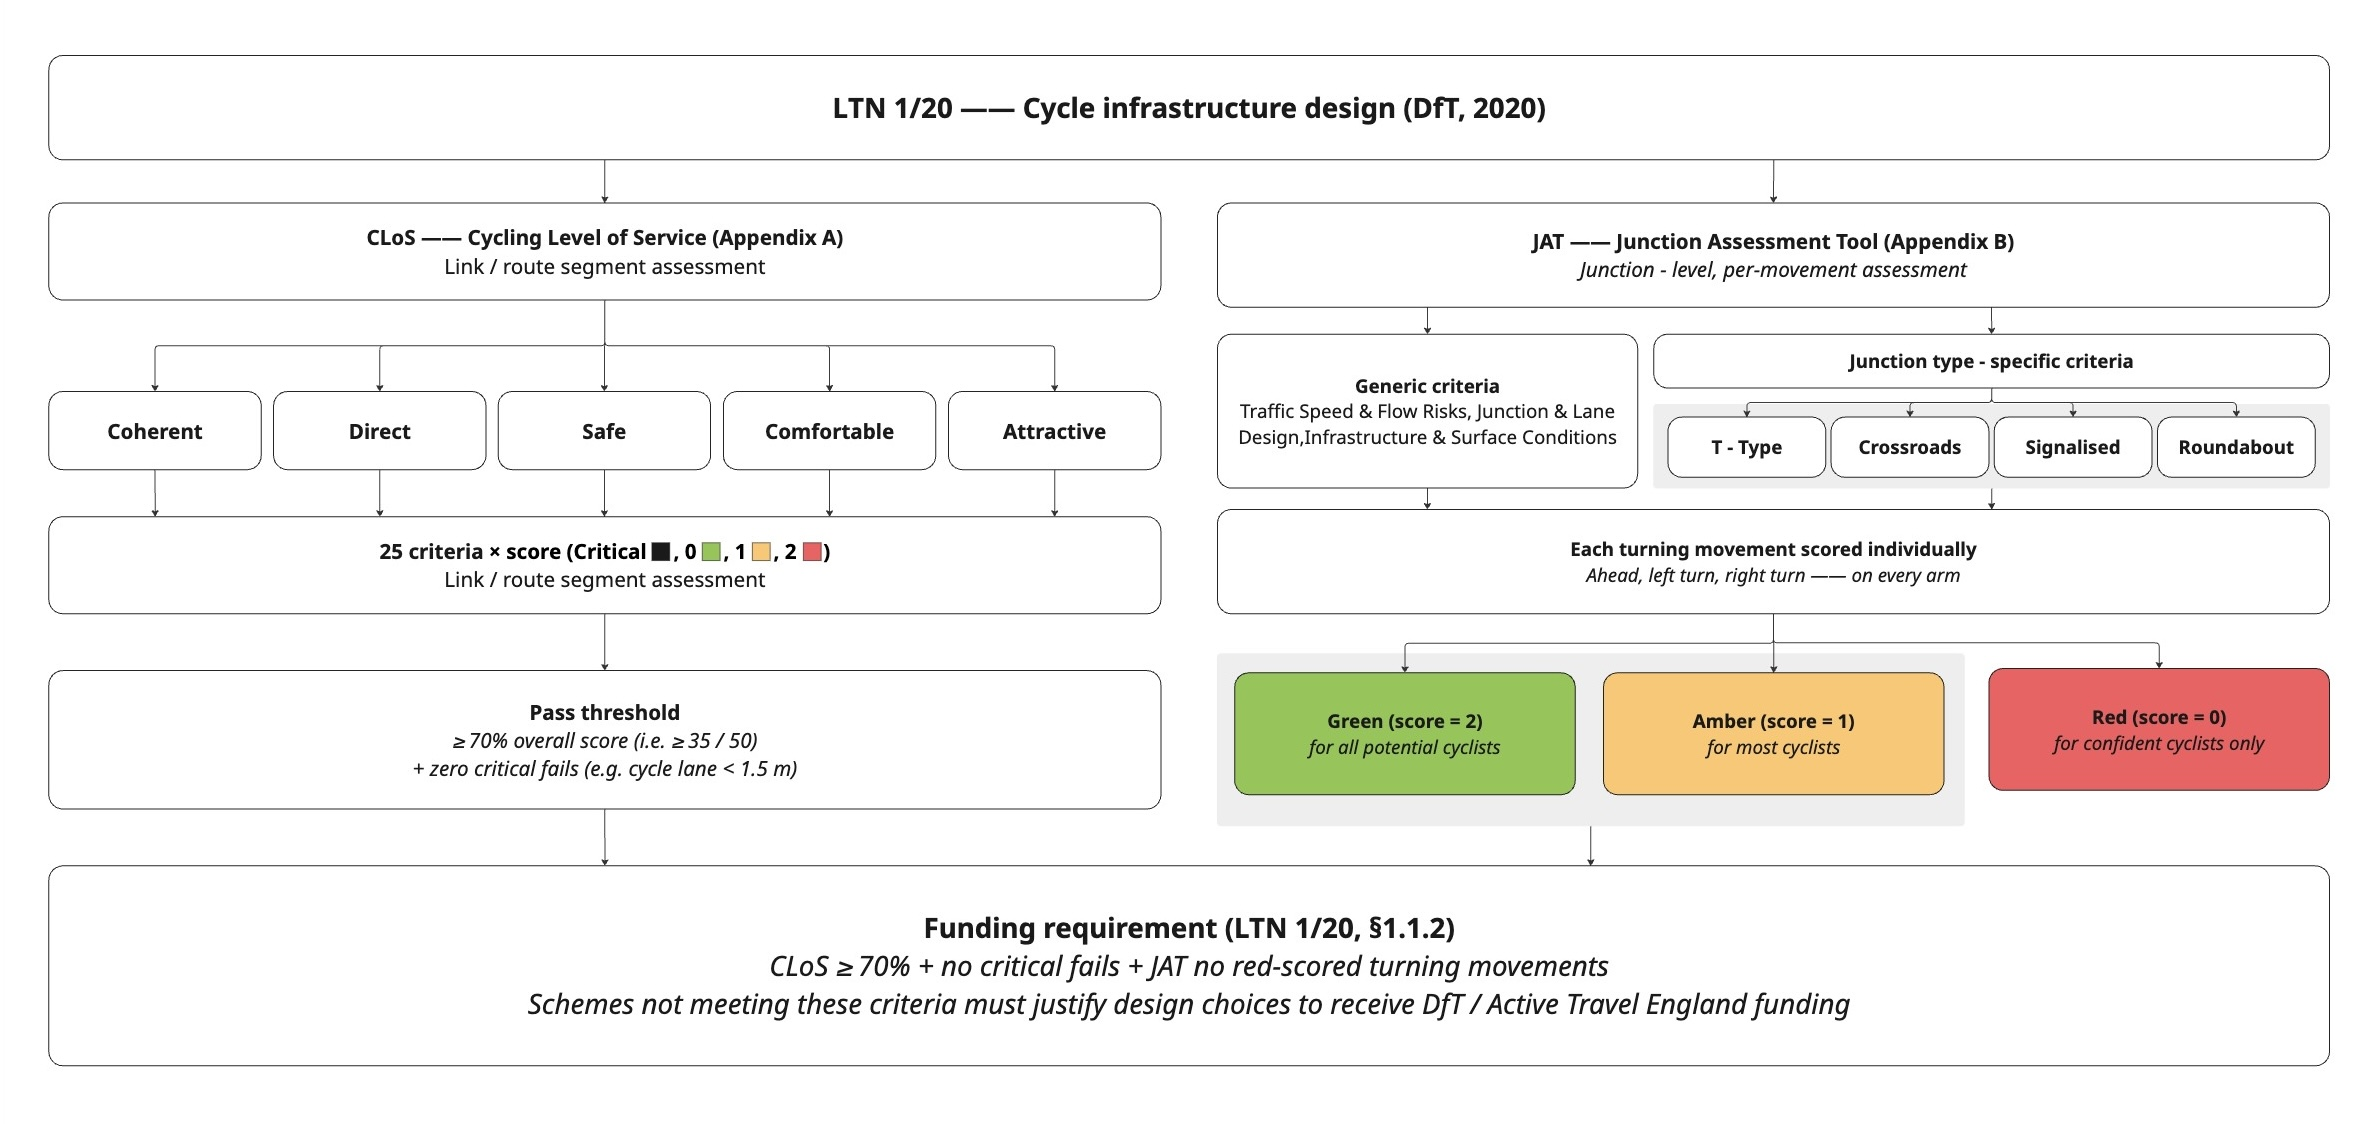
\includegraphics[width=\textwidth]{Figure/ltn.jpg}
    \caption{Structure of the LTN 1/20 evaluation framework, comprising the Cycling Level of Service (CLoS) and the Junction Assessment Tool (JAT), and their combined role in determining Active Travel England funding eligibility. Compiled by author from Department for Transport \textcite{departmentfortransport2020a}.}
    \label{fig:ltn}
\end{figure}

Despite this comprehensive coverage, LTN 1/20's evaluation tools present three structural limitations when considered as a framework for network-wide cycling assessment. Firstly, the CLoS and JAT are scheme-level audit instruments requiring on-site evaluation by trained assessors, an approach that cannot scale to the classification of all cyclable links across an urban network and that risks inconsistency where subcriteria demand qualitative judgement \parencite{hancock2024}. Secondly, the CLoS abandons the population-referenced framing that the JAT adopts for its scoring tiers, defining all 25 subcriteria in purely technical terms. This reflects a structural constraint: the subcriteria mix stress-determinant factors that do implicitly delineate population acceptability, such as motor traffic speed, volume, and segregation, with experience-quality factors that do not, such as wayfinding and cycle parking provision. Additive scoring methods of this kind are inherently compensatory, such that strong performance on one set of criteria can arithmetically offset weaknesses in another \parencite{pais2022,wang2022}; applied to CLoS, a link may therefore satisfy the 70\% threshold through strong performance on the latter while falling short on stress conditions that, though not critical failures, would nonetheless deter the majority of potential cyclists. Thirdly, while the CLoS includes coherence subcriteria that address route-level continuity, these assess attributes of individual links rather than the connectivity of the network as a whole. They cannot answer whether a cyclist can complete a journey from origin to destination entirely within tolerable traffic conditions, yet end-to-end low-stress connectivity between origins and destinations has been identified as the most fundamental determinant of whether a cycling network can attract the widest possible segment of the population \parencite{mekuria2012a,wang2016,lowry2017}.


\section{Level of Traffic Stress: Origins, Framework, and Applications }
\label{sec:lit-lts}

Where LTN 1/20 aspires to design for all from 8 to 80 but operationalises this through a broad composite of design criteria, the Level of Traffic Stress (LTS) framework \parencite{mekuria2012a} makes population acceptability the sole organising principle of its classification. Mekuria et al. operationalised this by adapting \citeauthor{geller2009}'s (\hyperlink{cite.geller2009}{\citeyear{geller2009}}) four-part population typology, the "strong and fearless," "enthused and confident," "interested but concerned," and "no way, no how," validated by \textcite{dill2013}, into an infrastructure classification. They subdivided Geller's "interested but concerned" to distinguish children from adults, yielding four LTS levels each anchored to a distinct population group: LTS 1 corresponds to children, demanding the greatest separation from traffic; LTS 2 to the mainstream "interested but concerned" adult majority, with criteria anchored to Dutch facility standards; LTS 3 to the "enthused and confident," comfortable with moderate traffic interaction; and LTS 4 to conditions tolerable only by the "strong and fearless" (Table~\ref{tab:lts-levels}). The "no way, no how," who would not cycle regardless of provision, have no corresponding level. To classify segments, LTS draws on the small number of road characteristics most directly associated with cycling stress, notably motor traffic speed, facility type and width, and the nature of intersection approaches and crossings, using readily observable attributes such as the number of traffic lanes as a proxy for variables like traffic volume that are rarely available at network scale \parencite{mekuria2012a,furth2016,furth2018,bearn2018}. Classification follows a non-compensatory rule: a segment's LTS is determined by its worst-performing attribute, so that a single high-stress condition is sufficient to determine the classification regardless of other favourable characteristics.

\begin{table}[htbp]
  \centering
  \caption{Level of Traffic Stress classification and corresponding population groups.}
  \label{tab:lts-levels}
  \begin{tabularx}{\textwidth}{l X}
    \toprule
    \textbf{LTS Level} & \textbf{Population Group and Description} \\
    \midrule
    LTS 1 & Suitable for almost all cyclists, including children cycling independently \\
    LTS 2 & Tolerable to the mainstream adult population; anchored to Dutch design standards proven to attract broad demographic participation \\
    LTS 3 & Tolerable to experienced cyclists who prefer dedicated space but accept moderate traffic interaction \\
    LTS 4 & Tolerable only to the strong and fearless riders willing to integrate with fast or heavy traffic \\
    \bottomrule
  \end{tabularx}
\end{table}

The original LTS framework proposed systematic network connectivity measures based on the population-anchored classification, quantifying the share of origin-destination pairs connected at each stress threshold and demonstrating how targeted gap closures can substantially multiply low-stress connectivity \parencite{mekuria2012a,furth2016}. This approach has since been widely adopted: a scoping review by \textcite{schon2024} identified 25 studies employing LTS to classify network links by stress level, primarily to measure cumulative accessibility by quantifying destinations reachable via low-stress links within defined distance or time thresholds \parencite{murphy2019,wasserman2019,gehrke2025}. Beyond cumulative measures, LTS-based analysis has been used to evaluate job accessibility through detour-ratio methods that permit travel on higher-stress links when low-stress routing is substantially longer \parencite{furth2016,lowry2017,cabral2019}, to assess transport equity by linking low-stress connectivity to socioeconomic indicators \parencite{tucker2018,kent2019}, and to identify network barriers and prioritise infrastructure investment \parencite{lowry2017,putta2019}. Collectively, LTS modelling and network filtering have become the dominant approaches in cycling accessibility and equity research \parencite{louro2026}.

Two limitations constrain the applicability of existing LTS implementations to the UK context. Firstly, all published criteria were calibrated to North American road design conventions, speed regimes, and infrastructure types, and no LTS classification grounded in UK design standards has been developed systematically. Although the framework has been applied to British cities \parencite{cervero2019,jeong2025}, these implementations relied on simplified criteria derived from North American conventions rather than national design guidance. Secondly, the progressive simplification of the original criteria for network-scale application has produced considerable methodological divergence, with \textcite{harvey2024} finding substantial disagreement across seven LTS methods applied to the same cities, underscoring the sensitivity of results to variable selection and threshold definitions. These two limitations motivate the approach taken in this study: rather than adapting any single North American LTS variant, the classification is grounded in LTN 1/20, a single national design standard that provides both the threshold structure and the population-acceptability logic needed to anchor an LTS classification to English conditions.


\section{Growing Fragmented Cycling Networks}
\label{sec:lit-networkgrowth}

Cycling networks in most cities remain sparse and fragmented \parencite{schoner2014,szell2022,reggiani2023}, so how they should expand, and in what order, is a live planning question. Network growth simulation addresses this by modelling expansion as the sequential addition of edges under a selection rule, generating investment trajectories whose connectivity outcomes can be compared \parencite{barthelemy2009,xie2009,szell2022}. Approaches to cycling network growth simulation can be divided by direction of construction: forward approaches iteratively add edges, either expanding from an existing network by bridging disconnected components \parencite{nateraorozco2020}, growing from scratch around topologically central seed points \parencite{szell2022}, or prioritising segments on the street network by potential routed cycling demand \parencite{mahfouz2023}. Inverse approaches begin from an idealised complete network and greedily remove the least important edges to generate budget-indexed subnetworks \parencite{steinacker2022}. Both directions can incorporate topological centrality \parencite{szell2022} or cycling demand to weight edge importance \parencite{steinacker2022,mahfouz2023}. A recurring finding is that how a fragmented network is grown matters as much as how much is built. \textcite{nateraorozco2020} show across fourteen cities that small, targeted investments connecting disconnected components rapidly consolidate a bicycle network, far outperforming random, uncoordinated addition, while \textcite{szell2022} find that uninformed growth needs several times the investment of a flow-based strategy before a connected network emerges. 

These studies operate on networks defined by infrastructure presence, in which an edge either belongs to the cycling network or does not, and they deploy growth simulation to identify an optimal expansion sequence. Neither feature carries over to a stress-classified network, where the object of investment is the upgrading of existing high-stress links, and low-stress conditions arise as much from quiet residential streets as from dedicated facilities.  

\section{Research Gap and Questions}
\label{sec:lit-gaprq}

The preceding review establishes three gaps at the intersection of design standards, network assessment, and investment planning. First, while LTN 1/20 provides the most comprehensive national design standard for cycling infrastructure in England, its evaluation instruments remain confined to scheme-level audit. The CLoS's compensatory scoring obscures the population-referenced acceptability that the standard's ``cycling for all'' principle implies, and neither the CLoS nor the JAT can assess whether compliant schemes cohere into a network that connects origins to destinations at tolerable stress levels (Section~\ref{sec:lit-ltn}), despite end-to-end low-stress connectivity being the most fundamental determinant of a network's capacity to attract the wider population \parencite{mekuria2012a,lowry2017}.

Second, the LTS framework supplies precisely the network-level, population-anchored logic that LTN 1/20's instruments lack, yet no published implementation is grounded in UK design standards. Existing applications to British cities rely on simplified adaptations of North American criteria \parencite{cervero2019,jeong2025}, and applied practice inherits further weaknesses from the Conveyal lineage: undirected max-propagation of junction stress and the absence of any treatment of roundabouts, a junction form both prevalent in the UK and associated with elevated cyclist risk (Section~\ref{sec:lit-lts}). The recent completion of the OS NGD Transport Cycle Lane collection removes the principal data barrier to a standards-grounded classification, but as a newly released dataset its completeness and reliability have not been independently assessed.

Third, the network growth literature demonstrates that the sequence of investment shapes connectivity outcomes as strongly as its volume, but existing simulations operate on networks defined by infrastructure presence, in which edges are added rather than upgraded (Section~\ref{sec:lit-networkgrowth}). Whether these findings transfer to a stress-classified network, where low-stress conditions arise as much from quiet streets as from dedicated facilities and the investment problem is one of reclassifying existing high-stress links, remains untested.

These gaps motivate the overarching aim of this dissertation: to develop and apply a network-level cycling infrastructure assessment grounded in English design standards. Three research questions structure the study:

\begin{description}
  \item[\textnormal{RQ1.}] How can the design criteria of LTN 1/20 be operationalised into a directed, network-scale Level of Traffic Stress classification, including junction and roundabout assessment, using OS NGD Transport data?
  \item[\textnormal{RQ2.}] To what extent does the West Midlands cycling network deliver the connected, low-stress conditions that LTN 1/20's ``cycling for all'' principle requires, for the population groups the standard identifies?
  \item[\textnormal{RQ3.}] How do alternative strategies for upgrading high-stress links compare in their capacity to improve low-stress network connectivity?
\end{description}

% ============================================================
% CHAPTER 3: STUDY AREA AND DATA
% ============================================================
\chapter{Study Area and Data}
\label{ch:data}

\section{Study Area: The West Midlands}
\label{sec:study-area}

The study focuses on the West Midlands metropolitan region. Located in central England, it comprises the seven metropolitan boroughs of Birmingham, Coventry, Dudley, Sandwell, Solihull, Walsall, and Wolverhampton. With a population of over 3 million \parencite{officefornationalstatistics2025}, the West Midlands is the second largest and second most populated conurbation in Britain after London \parencite{westmidlandscombinedauthority2025}. As Figure~\ref{fig:study-area} illustrates, the region exhibits a polycentric urban structure, with Birmingham as the dominant core surrounded by smaller but densely populated centres including Wolverhampton, Coventry, and the towns of the Black Country \footnote{The Black Country refers to the area immediately west and northwest of Birmingham, comprising the metropolitan boroughs of Dudley, Sandwell, Walsall, and Wolverhampton.}, While the southern and eastern portions of Solihull and the fringes of Walsall and Birmingham are predominantly rural. This mix of dense urban centres and lower-density peripheral areas presents distinct challenges for cycling infrastructure provision, as routes must negotiate fragmented land uses, varying traffic conditions, and considerable trip distances between centres \parencite{delclos-alio2024}.

\begin{figure}[h]
  \centering
  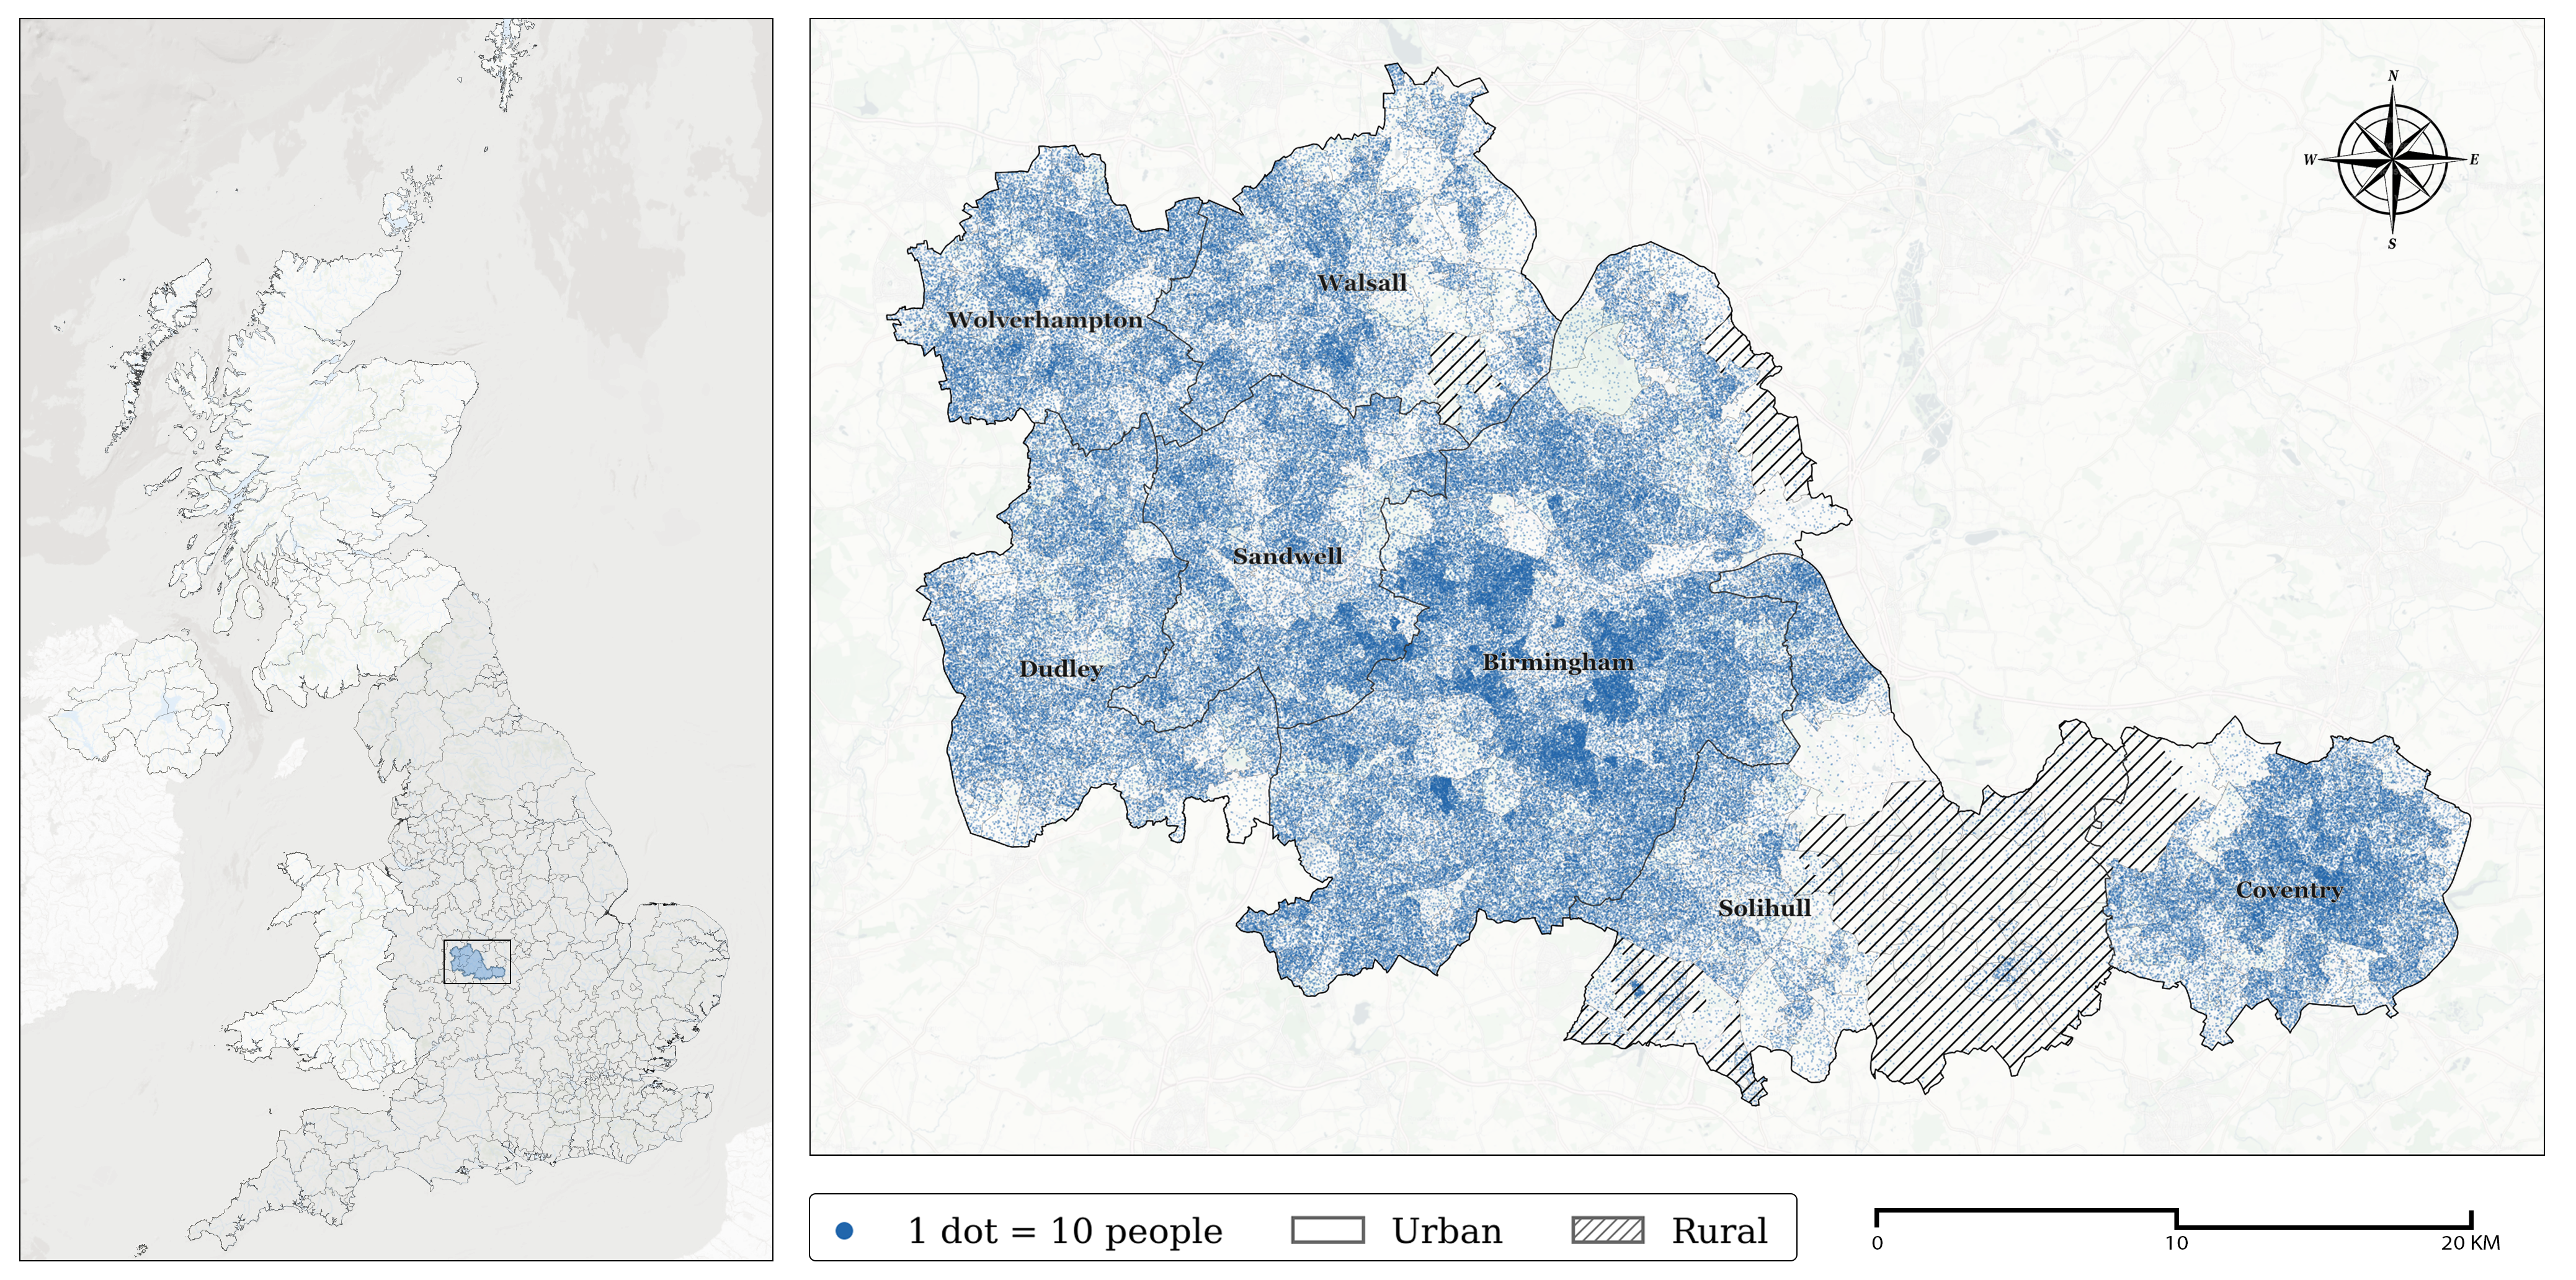
\includegraphics[width=\textwidth]{Figure/study_area_map.png}
  \caption[Study area: The West Midlands]{Study Area: The West Midlands.}
  \label{fig:study-area}
\end{figure}
 
The West Midlands has been a centre of British automobile manufacturing since the early twentieth century, accounting for approximately 60\% of national car production in the early 1970s \parencite{donnelly2017}. Its urban fabric bears this legacy: post-war interventions such as Birmingham's Inner Ring Road, completed in 1971 as Britain's first urban motorway \parencite{gunn2018}, entrenched car-oriented mobility across the region, exemplifying what \textcite{mattioli2020} characterise as a self-reinforcing car-dependent system. National Travel Survey data show that the wider West Midlands region \footnote{The wider West Midlands region includes the seven metropolitan boroughs as well as the surrounding counties of Herefordshire, Shropshire, Staffordshire, Warwickshire, and Worcestershire.} consistently records the highest share of private motorised trips among English regions, at 69\% in 2024 \parencite{departmentfortransport2025}. And cycling accounts for only approximately 0.9\% of all trips in the metropolitan area \parencite{westmidlandscombinedauthority2024}, despite 41\% of car journeys being under two miles \parencite{westmidlandscombinedauthority2019}. 

In response, Transport for West Midlands (TfWM) has set out an ambitious active travel agenda centred on the Starley Network, a planned 500-mile network of traffic-free or physically separated cycle routes \parencite{westmidlandscombinedauthority2020}, aligned with the national Gear Change vision and LTN 1/20 design standards. Yet the gap between this policy ambition and the region's measurable network-level cycling conditions remains poorly quantified, making the West Midlands a compelling case for the standards-based infrastructure assessment developed in this study.

\section{Data Sources: Overview}
\label{sec:data}

The analytical pipeline draws on four principal data sources. The primary source is Ordnance Survey National Geographic Database Transport (OS NGD Transport), which provides network geometry, road classification, carriageway and cycle lane width, legal access designation, junction type and probe-vehicle-derived average speeds for constructing the directed, stress-classified network (Sections~\ref{sec:method-extraction}--\ref{sec:method-junctionlts}). The Cycle Lane feature collection, achieving full national coverage in March 2026 \parencite{ordnancesurvey2026e}, makes this study one of the first to incorporate authoritative national cycling infrastructure data into a network-level assessment. Department for Transport road traffic count data supply observed AADT volumes and training observations for minor road volume estimation (Section~\ref{sec:method-linklts}). OpenStreetMap (OSM) contributes cycling geometries for Path Link cross-validation, traffic signal locations for junction classification, and school locations for accessibility analysis (Sections~\ref{sec:method-extraction}, \ref{sec:method-junctionlts}, \ref{sec:method-analysis}). Census data from the Office for National Statistics provide MSOA-level commuting flows for OD connectivity and network growth evaluations, and LSOA-level population and boundaries for density and reach analyses (Sections~\ref{sec:method-analysis}--\ref{sec:method-growth}). Table~\ref{tab:datasets} summarises each dataset.

\begin{table}[H]
  \centering
  \caption{Datasets used in this study.}
  \label{tab:datasets}
  \small
  \begin{tabularx}{\textwidth}{l l X l l}
    \toprule
    \textbf{Dataset} & \textbf{Provider} & \textbf{Key Variables} & \textbf{Spatial Unit}  \\
    \midrule
    Road Links        & OS NGD & Geometry, classification, description, width & Edge \\
    Path Links        & OS NGD & Geometry, cycle lane presence & Edge  \\
    Highway Dedication & OS NGD & Legal access designation & Edge  \\
    Cycle Lane        & OS NGD & Facility type, width, placement side & Edge  \\
    Average Speed (RAMI) & OS NGD & Probe-derived average speed & Edge  \\
    Road Node         & OS NGD & Node form, geometry, description & Node  \\
    Path Node         & OS NGD & Node geometry & Node  \\
    \midrule
    Road Traffic Counts & DfT  & AADT by vehicle type & Count point  \\
    \midrule
    Cycling Network   & OSM   & Highway and cycleway tags & Way  \\
    Traffic Signals   & OSM   & Signal node locations & Node  \\
    Schools           & OSM   & Location & Point  \\
    \midrule
    Commuting Flows   & ONS   & OD pairs within 8\,km & MSOA  \\
    Population        & ONS   & Resident population & LSOA \\
    Boundaries        & ONS   & LSOA/MSOA polygons & Polygon \\
    \bottomrule
  \end{tabularx}
\end{table}

\section{Statement of Ethics}
\label{sec:ethics}

This dissertation received ethical approval from the UCL Research Ethics Committee (reference: 3797). Ordnance Survey National Geographic Database data, licensed under the Public Sector Geospatial Agreement and not openly available, were provided by Transport for West Midlands under a formal data transfer agreement; all restricted datasets were stored on UCL-managed OneDrive. Semi-structured interviews with five transport practitioners were conducted with informed consent, and responses were fully anonymised in all outputs. No other personal or individually identifiable data were collected or processed.
% ============================================================
% CHAPTER 4: METHODOLOGY
% ============================================================
\chapter{Methodology}
\label{ch:methodology}

This chapter presents the analytical framework for classifying and evaluating the West Midlands cycling network by Level of Traffic Stress (Figure~\ref{fig:methods}). Sections~\ref{sec:method-extraction}--\ref{sec:method-junctionlts} construct the directed, stress-classified network: extracting cyclable segments from OS NGD, assigning link-level LTS, and propagating junction stress with LTN 1/20's criteria. Section~\ref{sec:method-analysis} uses this network to test connectivity against LTN 1/20's “Cycling for all” principle through density, fragmentation, and reach analyses. Section~\ref{sec:method-growth} compares three network growth strategies to inform upgrade prioritisation.

\begin{figure}[htbp]
  \centering
  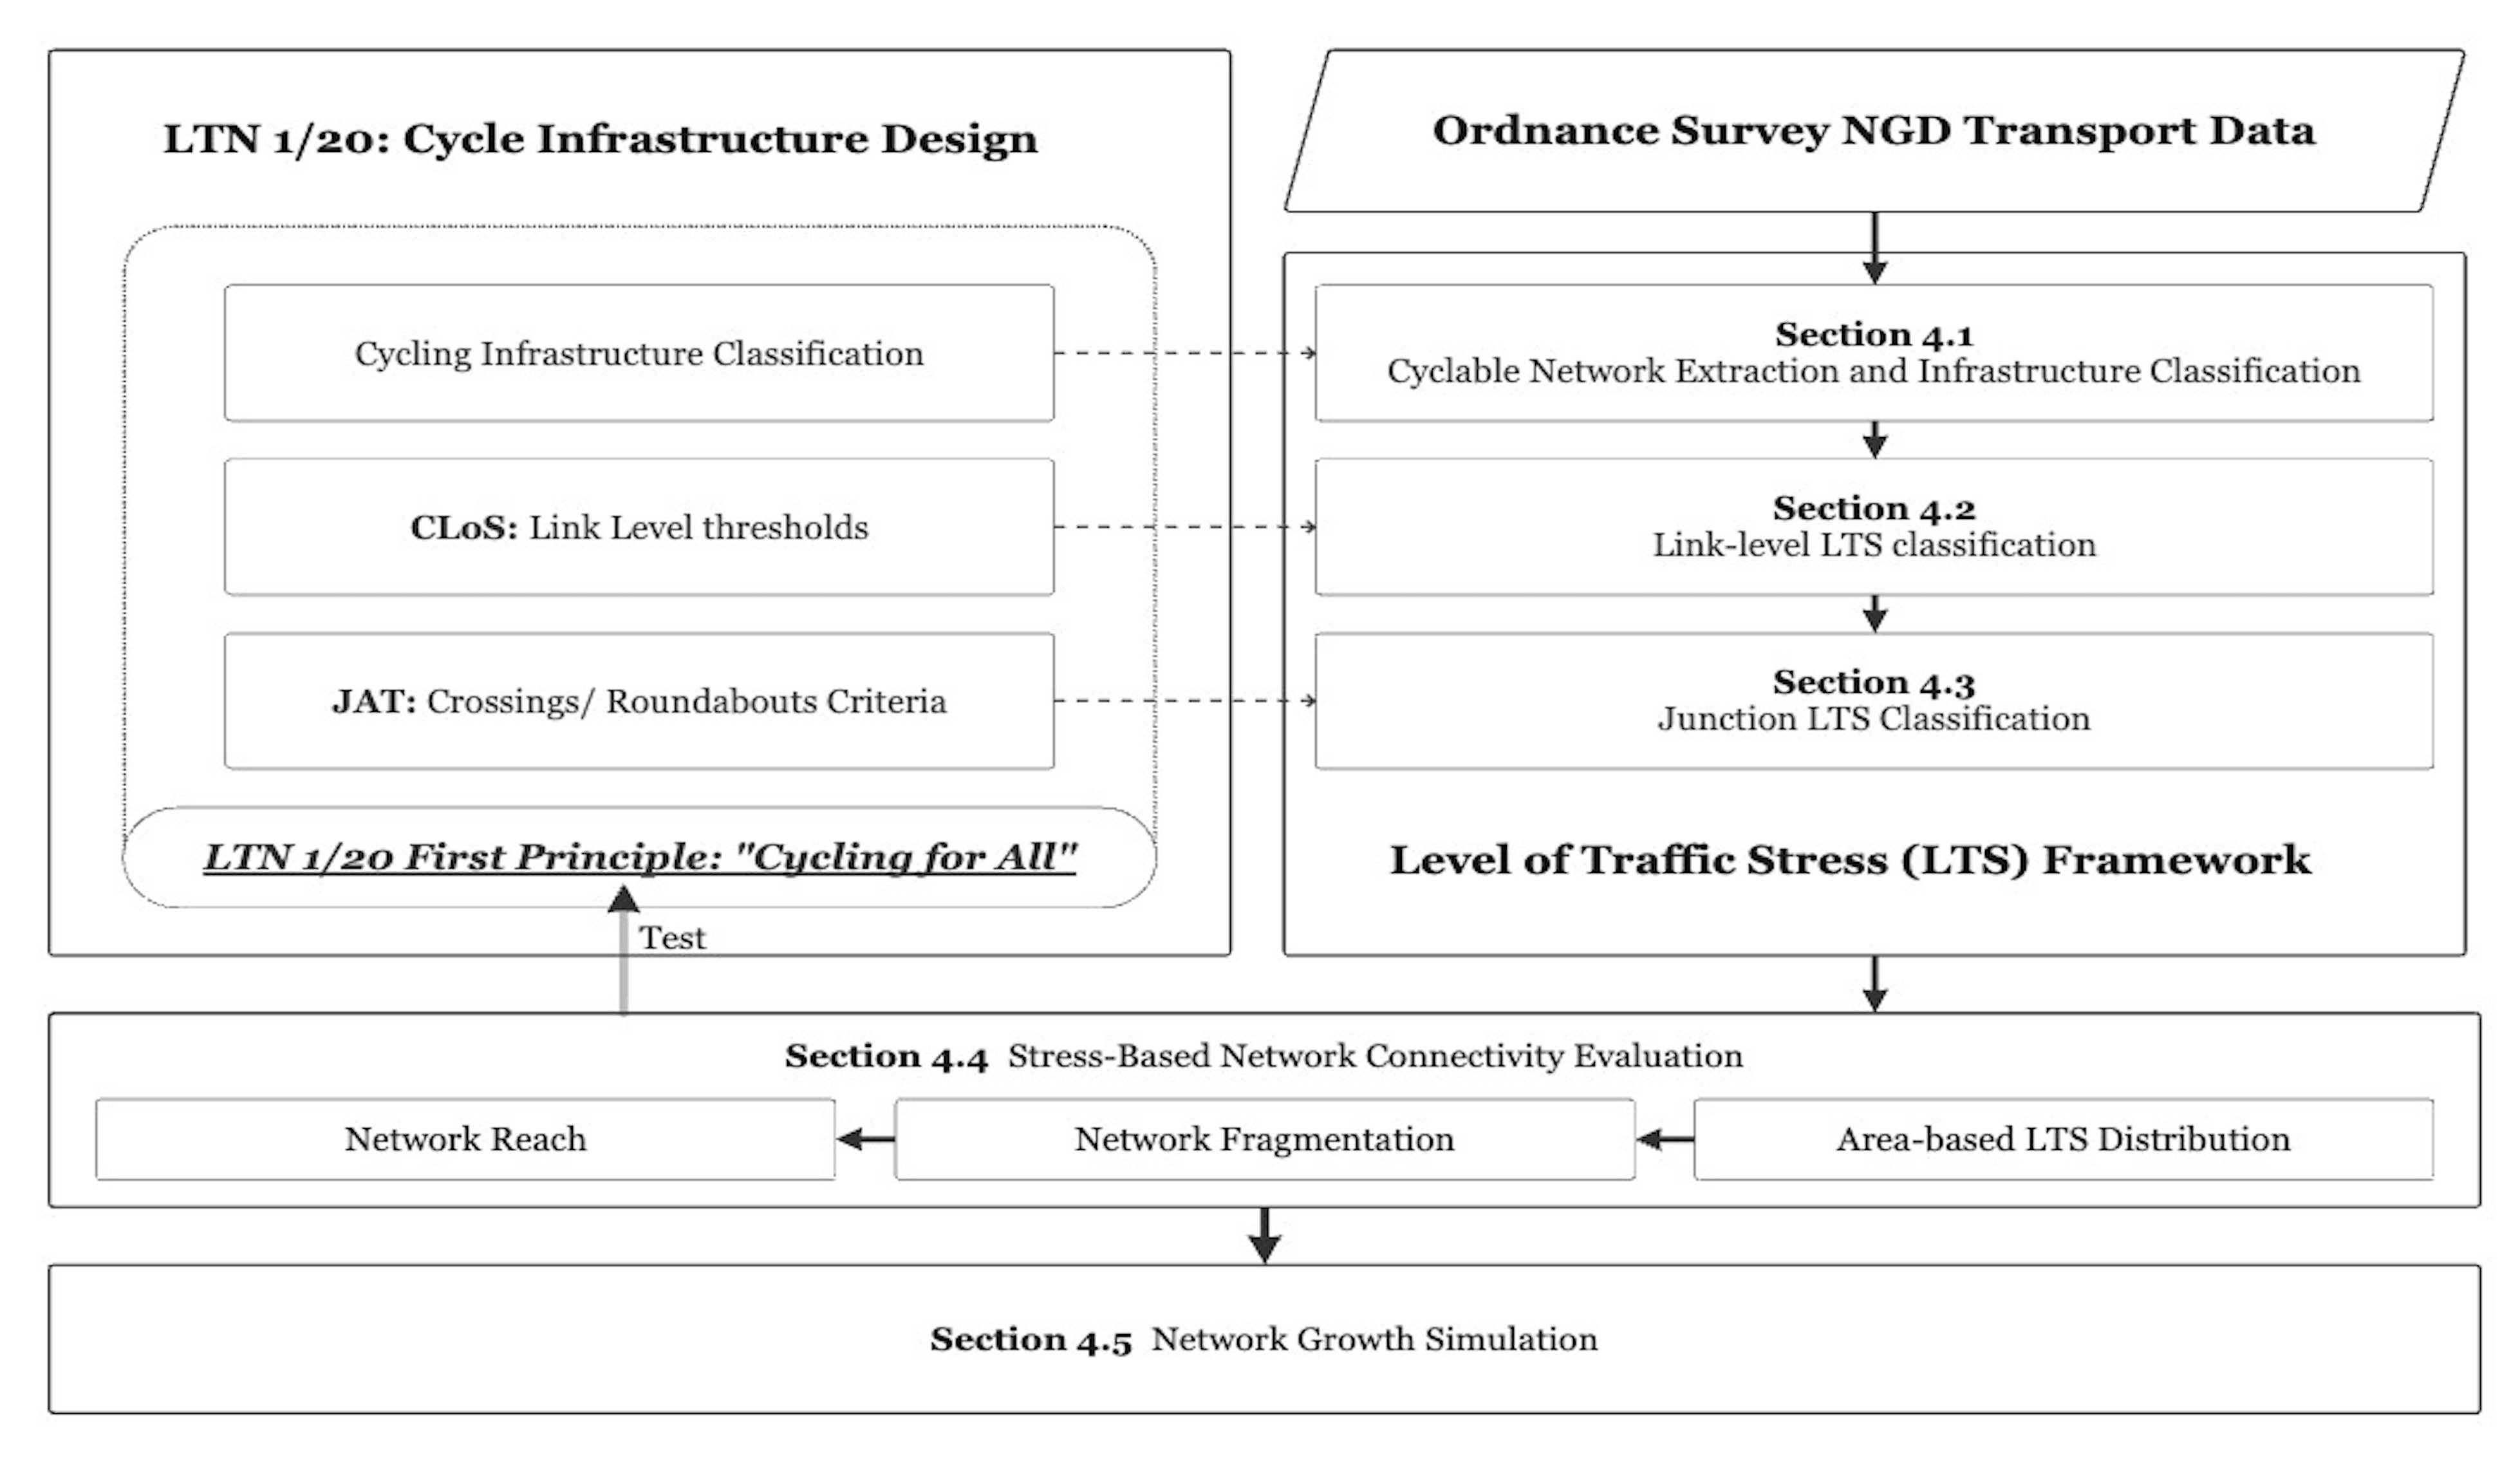
\includegraphics[width=\textwidth]{Figure/methods.jpg}
  \caption{Analytical framework. LTN 1/20 design criteria (left) supply the classification thresholds operationalised on OS NGD Transport data (right). The classified network is then evaluated against LTN 1/20's "Cycling for All" principle through connectivity analysis and network growth simulation.}
  \label{fig:methods}
\end{figure}

\section{Cyclable Network Extraction and Infrastructure Classification}
\label{sec:method-extraction}

The first stage of the classification process extracts all legally and practically cyclable segments from the West Midlands transport network. Cyclable infrastructure is represented in two feature collections under OS NGD Transport Theme: Road Links, which represent the carriageway network \parencite{ordnancesurvey2026a}, and Path Links, which represent routes topologically independent from it \parencite{ordnancesurvey2026b}. The legal cyclability of segments is firstly checked through the Highway Dedication feature collection, which provides an indication of the type of highway user who has access to each section of the network, recording one of eight designation types \parencite{ordnancesurvey2026}. Five of the seven designation types permit cycling under UK highway law, while `Motorway' and `Pedestrian Way Or Footpath' are excluded as non-cyclable (Table~\ref{tab:highway-dedication}).
 
\begin{table}[htbp]
  \centering
  \caption{Highway Dedication types and legal cyclability under UK highway law.}
  \label{tab:highway-dedication}
  \small
  \begin{tabularx}{\textwidth}{l l X}
    \toprule
    Highway Dedication & Cyclable? & Legal Basis \\
    \midrule
    All Vehicles & Yes & Cycling permitted on public roads by default \\
    Cycle Track or Cycle Way & Yes & Cycle Tracks Act 1984 \\
    Bridleway & Yes & Countryside Act 1968, s.30 \\
    Restricted Byway & Yes & Countryside and Rights of Way Act 2000 \\
    Byway Open to All Traffic & Yes & Wildlife and Countryside Act 1981, s.66(1) \\
    Motorway & No & Motorways Traffic (England and Wales) Regulations 1982 \\
    Pedestrian Way or Footpath & No & No public right of way for cycling (cf.\ Highways Act 1835, s.72) \\
    \bottomrule
  \end{tabularx}
  \par\smallskip
  \footnotesize\textit{Note:} The eighth type, `No Dedication Or Dedication Unknown', is neither cyclable nor explicitly non-cyclable and is addressed through the description-based fallback classification for Road Links.
\end{table}
 
For Road Links, Highway Dedication covers most of the segments. Where a dedication record is absent or recorded as `No Dedication Or Dedication Unknown', a fallback classification retains segments whose physical description feature indicates a carriageway type \footnote{`Single Carriageway', `Dual Carriageway', `Roundabout', `Slip Road', `Shared Use Carriageway', `Traffic Island Link At Junction', and `Traffic Island Link'.}. Segments classified as `Motorway' are excluded regardless of dedication status. This process yields 212,551 cyclable Road Links (97.8\%), of which 84.2\% are identified through Highway Dedication and 15.8\% through the description fallback. For Path Links, Highway Dedication coverage is substantially lower, identifying only 10.1\% of cyclable paths. A second layer retains paths where the feature data detects cycling infrastructure through its `presenceofcyclelane' attribute, contributing a further 1.0\%. No attribute in the OS NGD Path Link schema, however, provides a direct cyclability indicator. This mirrors DfT’s own transport connectivity metric, which uses Ordnance Survey data for the driving network but relies on OpenStreetMap tags for cycling and walking network definition \parencite{dft2025}. Following this, a third layer performs spatial cross-validation against the OpenStreetMap cycling network, matching remaining paths without Highway Dedication or cycle lane presence to OSM cycling geometries within a 5-metre nearest-neighbour spatial join and recovering an additional 40,035 paths. Paths with explicitly non-cyclable Highway Dedications are excluded at all layers. This process yields 45,023 cyclable Path Links (40.3\% of the total collection). Each segment is then expanded into directed edges, and cycle lane records are joined only to the edge whose travel direction aligns with the lane's placement side, capturing the inherently asymmetric distribution of cycling infrastructure and avoiding overestimation of facility provision.
 
Each directed cyclable segment is then classified into one of eight facility types derived from LTN~1/20's design hierarchy (Table~\ref{tab:facility-types}). The OS NGD Cycle Lane dataset, whose type definitions are aligned to LTN~1/20, records dedicated cycling infrastructure as separate features referencing their parent Road Link \parencite{ordnancesurvey2026c,ordnancesurvey2026d}. A Road Link with a matching Cycle Lane record is classified according to its cycle lane description; where multiple records exist for the same link, the more protective facility governs. Road Links without a matching record, or where the cycle lane type is recorded as `Unknown Type Of Cycle Track Or Lane', default to Mixed Traffic. All cyclable Path Links are classified as `Off-Road', as they are topologically independent from the road network and carry no motor traffic speed or volume attributes \parencite{ordnancesurvey2026b}. Following classification, Road Links and Path Links are merged into a single unified and directed network for use in the subsequent LTS assessment.
 
\begin{table}[h]
  \centering
  \caption{Facility type classification derived from LTN~1/20 design hierarchy, mapped to OS NGD data sources.}
  \label{tab:facility-types}
  \begin{tabular}{lll}
    \toprule
    Facility Type & OS NGD Source & Classification Feature \\
    \midrule
    Off-Road & Path Link & Cyclable Path Links \\
    Shared Use & Cycle Lane & `Unsegregated Shared Use Cycle Facility' / \\
     & & `Segregated Shared Use Cycle Track' \\
    Fully Kerbed Cycle Track & Cycle Lane & `Fully Segregated Cycle Track' \\
    Stepped Cycle Track & Cycle Lane & `Stepped Cycle Track Along Road' \\
    Light Segregation & Cycle Lane & `Lightly Segregated Cycle Lane On Road' \\
    Mandatory Cycle Lane & Cycle Lane & `Mandatory Cycle Lane On Road' \\
    Advisory Cycle Lane & Cycle Lane & `Advisory Cycle Lane On Road' \\
    Mixed Traffic & Road Link (main) & `Unknown Type Of Cycle Track Or Lane' or \\
     & & no matching Cycle Lane record \\
    \bottomrule
  \end{tabular}
  \par\smallskip
  \footnotesize\textit{Note:} Some facility types overlap conceptually. Off-Road paths may in practice function as shared-use routes or as kerbed cycle tracks. This does not affect the subsequent LTS classification, as all such facilities are fully separated from motor traffic.
\end{table}


\section{Link-level LTS classification}
\label{sec:method-linklts}

The link-level LTS classification adapts the \textcite{mekuria2012a} framework by replacing its North American thresholds with those from LTN~1/20. Although the CLoS tool uses compensatory scoring across heterogeneous subcriteria, which prevents it from isolating population-level acceptability (see Section~\ref{sec:lit-ltn}), the core Safety subcriteria addressing motor traffic speed (Criterion 10), volume (Criterion 11), segregation provision and carriageway width (Criterion 12) are themselves non-compensatory stress determinants constructed on CROW-derived logic \parencite{crow2016}, directly consistent with the LTS framework. This study maps that graduated logic onto the four LTS levels: conditions suitable for all users including children (LTS 1), most adults (LTS 2), confident cyclists (LTS 3), and conditions triggering a critical safety failure under LTN 1/20 criteria (LTS 4), as detailed in Table~\ref{tab:lts_matrix}.

\renewcommand{\arraystretch}{1.4}
\begin{table}[h]
\centering
\caption{Link-level LTS classification matrix derived from LTN~1/20 Safety subcriteria.}
\label{tab:lts_matrix}
\footnotesize
\begin{tabularx}{\textwidth}{
  >{\raggedright\arraybackslash}p{2.8cm}
  >{\raggedright\arraybackslash}X
  >{\raggedright\arraybackslash}X
  >{\raggedright\arraybackslash}X
  >{\raggedright\arraybackslash}X
}
\toprule
\textbf{Facility type} & \textbf{LTS~1} & \textbf{LTS~2} & \textbf{LTS~3} & \textbf{LTS~4} \\
\midrule
Off-Road              & All conditions & ---  & ---  & ---  \\
Shared Use            & All conditions & ---  & ---  & ---  \\
Fully Kerbed Cycle Track & All conditions & --- & --- & ---  \\[3pt]
Stepped cycle track   & $V_{85} \leq 30$\,mph & $V_{85}$ 30--37\,mph & $\geq 37$\,mph & --- \\
Light segregation     & $V_{85} \leq 30$\,mph & $V_{85}$ 30--37\,mph & $\geq 37$\,mph & --- \\[3pt]
Mandatory cycle lane  &
  Width $\geq 1.8$\,m,\newline $V_{85} \leq 20$\,mph,\newline AADT $\leq 5{,}000$ &
  Width $\geq 1.8$\,m,\newline $V_{85}$ 20--30\,mph,\newline AADT $\leq 5{,}000$ &
  Width $< 1.8$\,m; or\newline $V_{85}$ 30--37\,mph; or\newline AADT 5,000--10,000 &
  $V_{85} \geq 37$\,mph; or\newline AADT $\geq 10{,}000$ \\[3pt]
Advisory cycle lane   &
  Width $\geq 1.8$\,m,\newline $V_{85} \leq 20$\,mph,\newline AADT $\leq 5{,}000$ &
  Width $\geq 1.8$\,m,\newline $V_{85}$ 20--30\,mph,\newline AADT $\leq 5{,}000$ &
  Width $< 1.8$\,m; or\newline $V_{85}$ 30--37\,mph; or\newline AADT 5,000--10,000 &
  $V_{85} \geq 37$\,mph; or\newline AADT $\geq 10{,}000$ \\[3pt]
Mixed traffic         &
  $V_{85} \leq 20$\,mph,\newline AADT $\leq 2{,}500$ &
  $V_{85}$ 20--30\,mph,\newline AADT 2,500--5,000 &
  $V_{85}$ 30--37\,mph; or\newline AADT 5,000--10,000 &
  $V_{85} \geq 37$\,mph; or\newline AADT $\geq 10{,}000$; or\newline nearside lane 3.2--3.9\,m\newline and AADT $\geq 5{,}000$ \\
\bottomrule
\end{tabularx}

\vspace{0.5em}
\footnotesize
\noindent\textit{Notes:}
\begin{enumerate}[nosep, leftmargin=*, label=\arabic*.]
    \item Where multiple criteria apply to a single segment, the overall LTS is determined by the worst-performing criterion (non-compensatory).
    \item Thresholds are derived from the CLoS Safety subcriteria (Criteria 9--12, 15) in LTN~1/20 Appendix~A, supplemented by the speed--volume--facility matrix in Figure~4.1, which the CLoS itself references as complementary guidance for determining appropriate separation levels.
    \item Motor traffic volume is expressed as Annual Average Daily Traffic (AADT), used as a proxy for the passenger car unit (PCU) thresholds specified in LTN~1/20 Criterion~11. LTN~1/20 additionally specifies HGV composition thresholds ($>5\%$ for critical fail, 2--5\% for score~0); these could not be applied due to the absence of network-wide vehicle composition data and are acknowledged as a limitation (see section~\ref{sec:disc-limitations}).
    \item Rural exception: mixed traffic segments with $V_{85} \leq 30$\,mph and AADT $\leq 1{,}000$ are classified as LTS~1, following LTN~1/20 Figure~4.1 Note~3.
\end{enumerate}
\end{table}
\renewcommand{\arraystretch}{1.0}

The link-level LTS classification begins with facility type and proceeds through three primary variables: prevailing speed, road width, and motor traffic volume. OS~NGD provides carriageway or cycle lane width at the link level through average and minimum width attributes. For cycle lanes, this study uses the separately recorded modal lane width rather than the minimum, as it better captures typical conditions along a segment. For mixed traffic on single carriageways, average road width is used to assess the critical nearside lane width range of 3.2 to 3.9\,m associated with elevated close-pass risk\footnote{On one-way roads, total width serves directly as lane width; on two-way roads, lane width is approximated as half the total width, with the override applied only where AADT exceeds 5,000, as lower volumes allow drivers to overtake via the opposing lane.}. Segments triggering this override are classified as LTS~4.

Prevailing speed is represented by the estimated 85th percentile speed ($V_{85}$), consistent with the measurement basis specified in LTN~1/20. $V_{85}$ is preferred over posted speed limits as actual operating speeds frequently diverge from the limit depending on road geometry and enforcement, offering a more reliable measure of cycling stress \parencite{fitzpatrick2003, europeancommission2021, departmentfortransport2025b}. $V_{85}$ was estimated from the OS~NGD average speed dataset (RAMI), which provides mean vehicle speeds derived from probe vehicle data across multiple time periods. The mean of observed average speeds across all available time periods was used as the representative link speed, and $V_{85}$ was calculated by applying a 7/6 multiplier derived from CA~185 \textit{Vehicle speed measurement} \parencite{nationalhighways2019}, which defines $V_{85}$ as the mean speed plus one standard deviation and estimates the standard deviation as approximately one-sixth of the mean under the assumption of a normal speed distribution.

OS~NGD does not include motor traffic volume attributes. To address this, major road volumes were obtained directly from DfT annual average daily traffic (AADT) count point data, while minor road volumes were estimated following the methodology of \parencite{morley2016}. A Poisson GLM was constructed using road network characteristics extracted via pgRouting on the England OSM network as predictors and DfT count point observations as the dependent variable. Five-fold cross-validation ($n = 3{,}695$ count points) yields an $R^2$ of $0.604 \pm 0.019$ and Spearman's $\rho$ of $0.803 \pm 0.015$, considered sufficient for the coarse-grained LTS classification task. Predicted and observed AADT values were assigned to OS~NGD links via nearest-network spatial join. For the small number of links where no match was achieved, volume was imputed using the median AADT of the corresponding road classification to ensure network-wide coverage.

\section{Junction LTS Classification}
\label{sec:method-junctionlts}

The original LTS framework established intersection-specific criteria covering weaving conflicts and crossing stress, with junction stress propagated to approaching minor-street links \parencite{mekuria2012a,furth2016}. However, the fine-grained geometric data these require are unavailable at network scale \parencite{bearn2018,furth2018}, driving adoption of the \textcite{conveyal2015} method, which propagates the highest segment LTS at each unsignalized vertex to all incident edges without independently evaluating crossing geometry. This max-propagation logic has been widely applied \parencite{semler2017,murphy2019,huertas2020}, with variants introducing signal or stop sign presence as downgrading modifiers \parencite{bearn2018,lin2021}; a substantial number of studies omit junction treatment entirely \parencite{wang2022,viero2025}. Two gaps persist. First, all existing criteria address North American junction typologies and none cover roundabouts, despite their prevalence in UK networks and documented cyclist collision risk \parencite{daniels2009,aldred2021,poudel2021,rodrigues2022}. Second, undirected vertex-level propagation assigns elevated stress indiscriminately to all incident edges regardless of legal travel direction, obscuring heterogeneity in crossing conditions.

The Junction Assessment Tool (JAT) within LTN 1/20 evaluates junction suitability by
establishing criteria for each junction form (priority T-junction, crossroads,
traffic signals, roundabout), disaggregated by the specific cycle movement being
assessed. From this structure, three variables can be identified as governing
crossing stress: the speed and volume of conflicting motor traffic, which determine
the severity of the potential conflict; the number of lanes to be crossed in one movement,
which determines the duration of exposure; and the availability of protection such
as a central refuge, traffic signals, or dedicated cycle priority. LTN 1/20 also
provides a crossing design suitability matrix that classifies crossings by these
variables into three suitability tiers: suitable for most people, not suitable for
all, and suitable for few. For non-roundabout crossing junctions
(Table~\ref{tab:crossing-lts}), the present study maps these three suitability tiers
to LTS 1, LTS 2, and LTS 3--4 respectively. Protection is operationalised in three
levels: uncontrolled, traffic island (identified from the OS NGD link description
field ``Traffic Island Link At Junction\footnote{The OS NGD does
not distinguish between median refuges, central islands, and other refuge forms, but
the presence of a traffic island at a junction at minimum serves to channelise
traffic flow and provide physical separation.}''), and signalized (identified from
OpenStreetMap traffic signal tags spatially joined to OS NGD nodes).  For roundabouts
(Table~\ref{tab:roundabout-lts}), the classification is derived directly from the JAT
roundabout-specific criteria, which assess suitability by traffic throughput,
approach geometry, and off-carriageway cycle facility provision. Each roundabout is classified by the maximum AADT, V85, and road width of its incident links.

\begin{table}[htbp]
  \centering
  \caption{Crossing Junction LTS Classification}
  \label{tab:crossing-lts}
  \begin{tabularx}{\textwidth}{X X X c c c}
    \toprule
    & & & \multicolumn{3}{c}{LTS by protection level} \\
    \cmidrule(lr){4-6}
    V85 (mph) & AADT & Est.\ lanes & Uncontrolled & Traffic island & Signalised \\
    \midrule
    $\geq$ 37   & Any            & Any      & 4 & 4 & 3 \\
    30--37      & $>$ 10,000     & Any      & 4 & 4 & 1 \\
    30--37      & 6,000--10,000  & $\geq$ 2 & 4 & 4 & 1 \\
    30--37      & $\leq$ 6,000   & $\geq$ 2 & 3 & 3 & 1 \\
    30--37      & $\leq$ 10,000  & 1        & 2 & 2 & 1 \\
    $\leq$ 30   & $>$ 8,000      & $>$ 2    & 4 & 3 & 1 \\
    $\leq$ 30   & $>$ 8,000      & $\leq$ 2 & 3 & 2 & 1 \\
    $\leq$ 30   & 4,000--8,000   & $\geq$ 2 & 2 & 2 & 1 \\
    $\leq$ 30   & 4,000--8,000   & 1        & 2 & 1 & 1 \\
    $\leq$ 30   & $\leq$ 4,000   & $\geq$ 2 & 2 & 1 & 1 \\
    $\leq$ 30   & $\leq$ 4,000   & 1        & 1 & 1 & 1 \\
    \bottomrule
  \end{tabularx}
\end{table}

\begin{table}[htbp]
  \centering
  \caption{Roundabout LTS Classification}
  \label{tab:roundabout-lts}
  \begin{tabularx}{\textwidth}{X c}
    \toprule
    Base conditions & LTS \\
    \midrule
    AADT $>$ 8,000 AND est.\ lanes $\geq$ 2; OR V85 $\geq$ 37 mph & 4 \\
    AADT $>$ 8,000 OR est.\ lanes $\geq$ 2 (but not both)         & 3 \\
    All other roundabouts (compact/mini, AADT $\leq$ 8,000)       & 2 \\
    Segregated cycle facility AND traffic signal                  & 1 \\
    \bottomrule
  \end{tabularx}

  \smallskip
  {\footnotesize \textit{Note.} When traffic lights are present, the LTS value is
  reduced by one level to a minimum of LTS 2.}
\end{table}

The junction classification operates at the (link, junction node) pair level. The
JAT defines junction stress in terms of cycle movements ``in potential conflict''
with motor traffic, where conflict arises from traffic streams that cross or run
alongside the cyclist's path without being separated physically or in time.
Following this definition, the present study identifies conflicting links at each
crossing junction via the OS NGD directionality attribute, retaining only those that
a cyclist departing the node could legally enter, and further excluding straight-line
continuations of the approach link through a bearing-based filter (departure bearing
within $180^{\circ} \pm 30^{\circ}$, a threshold following the orientation criterion in
\textcite{mekuria2012a}). The three crossing variables (maximum V85, maximum AADT,
and maximum estimated lane count) are then taken from the remaining conflict links,
ensuring all three reflect the transverse traffic stream being crossed. For
roundabout nodes, where circulatory geometry renders approach-level analysis
inapplicable, the classification operates at the node level using the maximum
traffic attributes across all incident links. In both cases, the junction LTS is
overlaid onto the segment classification using worst-indicator-wins logic, so that
junction stress can only elevate the final LTS of a link.

\section{Stress-Based Network Connectivity Evaluation}
\label{sec:method-analysis}

The following analyses evaluate whether the West Midlands network delivers on the LTN 1/20 ``cycling for all'' principle by testing connectivity at LTS 1 (children and older adults) and LTS $\leq$ 2 (mainstream adults), with LTS $\leq$ 3 and $\leq$ 4 included for comparison \parencite{mekuria2012a,departmentfortransport2020a}. Following \textcite{viero2025} and \textcite{schon2024}, the evaluation proceeds through area-based distribution, network fragmentation and network reach.

\textbf{Area-based LTS distribution} Network density is computed at LSOA level as absolute density (km of LTS-classified network per km\textsuperscript{2}) and relative density (proportion of total road network at each LTS level). These metrics characterise the spatial supply of low-stress infrastructure independent of whether it forms a connected network.

\textbf{Network fragmentation} To assess route continuity, connected component analysis is applied: for each cumulative LTS threshold, edges exceeding the threshold are removed and connected components are identified from the undirected projection. The largest connected component (LCC)---the maximum contiguous network a cyclist can traverse without exceeding a given stress threshold---and its share of sub-network length measure network cohesion. The component size distribution and the relationship between network length and fragmentation are examined across the full cyclable network (10,634.6~km). Precise fragmentation metrics are additionally computed on the LCC of the full network, excluding topologically isolated stub segments so that measured fragmentation reflects the breaking of connected routes rather than pre-existing disconnection.

\textbf{Network reach} Network reach is defined as the total length of network reachable from a given origin within a distance threshold \parencite{peponis2008,feng2019,viero2025}. The analysis adopts an 8~km (5~miles) threshold, the distance within which 70\% of personal trips in England fall \parencite{departmentfortransport2020a,departmentfortransport2025}. For each cumulative LTS subgraph, Dijkstra shortest paths are computed on the directed graph from the nearest network node to each LSOA centroid to all reachable nodes within this threshold. To test demand-relevant connectivity, two OD analyses are applied additionally. School accessibility routes from each LSOA centroid to its nearest school (OpenStreetMap), and commuting connectivity uses Census 2011\footnote{The 2021 Census was conducted during the COVID-19 pandemic, when widespread home-working guidance significantly distorted commuting patterns. The 2011 Census is therefore adopted as a more representative baseline of routine commuting flows.} MSOA flows filtered to straight-line distances $\leq$ 8~km, computing the proportion of OD pairs and flow volume for which a route exists at each threshold. Following \textcite{viero2025}, gaps of up to 30~m between edges of the same LTS level are closed with bidirectional bridging edges to compensate for geometric imprecision in infrastructure mapping \parencite{schoner2014}.

\section{Network Growth Simulation}
\label{sec:method-growth}

As established in Section~\ref{sec:lit-networkgrowth}, the order in which a fragmented network is upgraded shapes its connectivity outcome. This section adopts a forward growth framework, adding edges to the existing stress-classified network rather than pruning an idealised one, since the starting condition and policy question are both defined by incremental upgrade from the current state. Rather than prescribing which links to upgrade, the analysis compares how alternative selection logics shape connectivity growth, treating the comparison as a diagnostic of how much selection logic alone determines network-level return.

The simulation operates on an undirected projection of the LTS-classified
network, where each undirected edge takes the worse LTS classification of its
two directions, ensuring that both directions must meet the LTS 2 standard for
the edge to be considered a low-stress link. This projection yields 255,286
undirected edges, of which 187,370 (73.4\%) are low-stress (LTS $\leq$ 2),
forming the initial low-stress subnetwork, and 67,916 (26.6\%) are high-stress
(LTS 3--4), forming the candidate pool for upgrade. Three strategies are tested,
spanning a topology-to-demand axis (Table~\ref{tab:strategies}). All strategies
share the same forward growth mechanism: at each step, one candidate edge is
selected according to the active strategy, reclassified as low-stress, and
added to the subnetwork.

\begin{table}[htbp]
  \centering
  \caption{Edge selection strategies for the network growth simulation.}
  \label{tab:strategies}
  \begin{tabularx}{\textwidth}{@{}p{2.1cm} >{\RaggedRight\arraybackslash}X p{2.3cm} p{2.7cm}@{}}
    \toprule
    Strategy & Selection Logic & Information Input & Reference \\
    \midrule
    Random
      & Uniform random from all candidates; 10 runs averaged
      & None
      & Null baseline \\[4pt]
    Connectivity
      & Prioritise adjacent edges merging distinct components, favouring the
        largest component; ties broken by shortest length
      & Network topology
      & Adapted from \textcite{nateraorozco2020} \\[4pt]
    Betweenness Centrality (BC)
      & Highest pre-computed edge BC from all candidates
      & Topological demand proxy
      & \textcite{szell2022}; \textcite{steinacker2022} \\
    \bottomrule
  \end{tabularx}
\end{table}

The random baseline provides a null expectation by selecting edges without
prior information, averaged over 10 independent runs. The connectivity strategy
greedily expands the LCC by prioritising adjacent edges that merge distinct
components, adapted from the component-merging logic of \textcite{nateraorozco2020}
but operating at single-edge granularity. Edge betweenness centrality is
computed on the full undirected street network using Networkit's parallelised
Brandes algorithm \parencite{staudt2016}, serving as a topological proxy for
latent cycling demand \parencite{mccahill2008,kirkley2018,szell2022}. Two
metrics are computed at regular intervals during the growth process. LCC share
is the total length of the largest connected component divided by the total
length of the current low-stress (LTS $\leq$ 2) subnetwork, measuring the
topological integration of the network. Demand-weighted connectivity is the
share of commuting flow whose origin and destination fall within the same
connected component of the low-stress subnetwork, using the same Census 2011
MSOA commuting data and 8\,km distance filter described in Section~\ref{sec:method-analysis}.

% ============================================================
% CHAPTER 5: RESULTS
% ============================================================
\chapter{Results}
\label{ch:results}

% Handbook: be selective; provide a narrative, not result after result.

\section{Network Composition and LTS Distribution}
\label{sec:results-composition}

\section{Data Source Comparison}
\label{sec:results-comparison}

\section{Fragmentation}
\label{sec:results-fragmentation}

\section{Reach and Accessibility}
\label{sec:results-reach}

\section{OD Connectivity}
\label{sec:results-od}

\section{Network Growth Simulation}
\label{sec:results-growth}

% ============================================================
% CHAPTER 6: DISCUSSION
% ============================================================
\chapter{Discussion}
\label{ch:discussion}

This chapter interprets the results in relation to the research aims and wider literature. Section~\ref{sec:disc-cyclingforall} evaluates the West Midlands network against LTN 1/20's "cycling for all" principle, situating the connectivity findings within evidence on cycling demand and mode share. Section~\ref{sec:disc-junction} examines junction stress as a structural mechanism of low-stress network severance, distinguishing the barrier roles of crossings and roundabouts. Section~\ref{sec:disc-planning} draws implications from the growth simulation for investment prioritisation and cross-authority coordination. Section~\ref{sec:disc-osvalidation} assesses OS NGD cycle lane data through a first independent comparison with OpenStreetMap, and Section~\ref{sec:disc-limitations} discusses limitations and directions for future work.

\section{Evaluating "Cycling for All": Network Connectivity Against LTN 1/20 Objectives}
\label{sec:disc-cyclingforall}

\section{Junction Stress and the Structural Severance of the Low-Stress Network}
\label{sec:disc-junction}

\section{Network Growth and Implications for Investment Coordination}
\label{sec:disc-planning}

\section{Assessing OS NGD Cycle Lane Data: A First Independent Comparison with OpenStreetMap}
\label{sec:disc-osvalidation}

% TODO: include the honest treatment of the Furth et al. (2026)
% primal-graph junction stress propagation critique; OS NGD
% cycle lane undercount and dataset maturity.

\section{Limitations and Future Work}
\label{sec:disc-limitations}

% ============================================================
% CHAPTER 7: CONCLUSION
% ============================================================
\chapter{Conclusion}
\label{ch:conclusion}

This dissertation set out to address the absence of a data-driven, network-level methodology for evaluating cycling infrastructure quality in England. While LTN~1/20 established the most comprehensive national design standards to date, its evaluation instruments were conceived for scheme-level audit and cannot assess whether a city's network, taken as a whole, delivers the connected low-stress conditions that its ``cycling for all'' principle requires. In response, this study developed a directed Level of Traffic Stress classification grounded entirely in LTN~1/20's own criteria and applied it to the West Midlands using the newly released OS NGD Transport data.

The contributions of this study span methodology and data. Methodologically, the classification replaces North American LTS thresholds with those derived from the CLoS Safety subcriteria, the JAT and the design criteria, producing the first LTS framework calibrated to English design standards and thereby restoring the population-anchored logic that LTN~1/20's compensatory scoring obscures. The directed network representation and bearing-based junction assessment further extend LTS practice beyond undirected max-propagation, incorporating roundabout-specific criteria absent from all prior implementations. On the data side, the study provides the first independent assessment of the OS NGD Cycle Lane dataset, establishing both its strengths in recording separated infrastructure and its systematic undercapture of paint-only provision, an evaluation that conditions the reliability of any future research built on this data source.

The findings demonstrate that abundant low-stress length does not constitute a usable network. Although low-stress segments dominate the West Midlands network by length, they fragment into ten thousands of disconnected components, with the largest contiguous low-stress network representing a small fraction of the whole. Arterial roads emerge as the primary source of severance, imposing high stress both along their links and at the junctions where low-stress residential clusters must cross them; this junction-level stress concentrates at the topological bottlenecks between clusters, while roundabouts function as near-absolute points of severance. The reach analysis makes the consequence tangible at the level of the individual cyclist: where on-carriageway provision lacks physical segregation, reachable distance without exceeding low-stress conditions collapses to that of the immediate residential cluster, terminating where the first arterial crossing is encountered. The result is that neither children nor mainstream adults can rely on the network for everyday journeys: only 4.1\% of the region's population can reach their nearest school via LTS~1 routes, and only 13.0\% of inter-MSOA commuting flow is connected via LTS~2 routes, with connected journeys requiring substantial detours.

These findings carry direct implications for investment practice. The growth simulation shows that the sequence of upgrades shapes connectivity outcomes as strongly as their total extent, with a strategy targeting component-bridging edges reaching connectivity milestones in roughly half the upgrade length of uninformed selection. This exposes a gap in the current policy architecture: LTN~1/20's funding-eligibility tools evaluate individual schemes, yet the connectivity of the network depends on where and in what order schemes are delivered, a coordination problem that scheme-level appraisal cannot resolve.

Because both the classification thresholds and the underlying data are national in scope, the framework can be applied to any English city without recalibration, enabling systematic benchmarking of network conditions against a single statutory standard. Future work should validate the classification against cyclist-perceived stress, extend junction assessment through movement-level dual-graph representations, and incorporate cost and equity dimensions into growth modelling. Ultimately, this dissertation demonstrates that LTN~1/20 contains within itself the material for its own network-scale evaluation. By translating its design criteria into a stress classification, the standard can be turned back upon the networks it governs, revealing in quantitative terms the distance between the ambition of cycling for all and the infrastructure through which that ambition must be realised.


% ---------- Bibliography ----------
\clearpage
\printbibliography[heading=bibintoc, title={Bibliography}]

% ---------- Appendices ----------
\appendix
% ============================================================
% APPENDIX B: SUPPLEMENTARY MATERIAL
% ============================================================
\chapter{Supplementary Material}
\label{app:supplementary}

\section{Traffic Volume Prediction}
\label{app:traffic-volume}

% TODO: Poisson GLM specification, AADT estimation details, etc.

\section{OSM and OS Birmingham Comparison}
\label{app:osm-os-comparison}

% TODO: cycle lane coverage comparison (63 km OS NGD vs 255 km OSM vs 139 km TfWM), etc.

\section{LTN 1/20's CLoS Web Assessment Tool for West Midlands}
\label{app:clos-tool}

% TODO: screenshots, architecture, link to zhengpei-xu.github.io/ltn1-20-assessment-tool-wm

% ============================================================
% APPENDIX A: RESEARCH LOG  (required, handbook 3.7)
% Must include dates of supervision meetings and at least one
% sentence describing what was discussed at each meeting.
% ============================================================
\chapter{Research Log}
\label{app:research-log}

\begin{longtable}{>{\raggedright\arraybackslash}p{2.5cm}
                  >{\raggedright\arraybackslash}p{3.5cm}
                  >{\raggedright\arraybackslash}p{8cm}}

\toprule
\textbf{Date} & \textbf{Type} & \textbf{Summary} \\
\midrule
\endfirsthead

\toprule
\textbf{Date} & \textbf{Type} & \textbf{Summary} \\
\midrule
\endhead

\midrule
\multicolumn{3}{r}{\textit{Continued on next page}} \\
\endfoot

\bottomrule
\endlastfoot

16/02/2026 & Stakeholder Collaboration & GeoDS project with TfWM confirmed. Contacts: Callum Bick, Charmaine Grant. \\
\addlinespace

05/03/2026 & Dissertation Development & \textbf{Supervision Meeting.} LTN criteria translation feasibility. \\
\addlinespace

20/03/2026 & Dissertation Development & \textbf{Supervision Meeting.} Start background reading of LTS framework. \\
\addlinespace

\multirow{2}{*}{13/04/2026} & Stakeholder Collaboration & \textbf{TfWM Meeting.} Detecting subjective LTN criteria; intro to LTS framework; signing data transform files. \\
 & Dissertation Development & \textbf{Supervision Meeting.} Filling ethics forms meeting. \\
\addlinespace

\multirow{2}{*}{22/04/2026} & Stakeholder Collaboration & TfWM Datasets received; checking for completeness and coverage \\
 & Dissertation Development &  UCL ethics forms in progress: screening, data protection \\
\addlinespace

\multirow{2}{*}{08/05/2026} & Stakeholder Collaboration & \textbf{TfWM Meeting.} Showing potential results of LTS framework with OSM. \\
 & Dissertation Development & \textbf{Supervision Meeting.} Reproduce paper with OSM for London and West Midlands. \\
\addlinespace

\multirow{2}{*}{18/05/2026} & Stakeholder Collaboration & \textbf{TfWM Meeting.} Three deliverables confirmed, mid-term report. \\
 & Dissertation Development & \textbf{\href{https://github.com/zhengpei-xu/PCTNI}{PCTNI Hackathon},} Queen's University Belfast (Prof.\ Robin Lovelace). LTS and connectivity analysis applied to Belfast cycle network. \\
\addlinespace

29/05/2026 & Stakeholder Collaboration & \textbf{TfWM Meeting.} Making planning for stakeholder interviews. \\
\addlinespace

\multirow{2}{*}{18/06/2026} & Stakeholder Collaboration & \textbf{TfWM Meeting.} Conducted 4 interviews so far; generating initial stakeholder insights. \\
 & Dissertation Development & \textbf{Supervision Meeting.} Building LTS-England with LTN 1/20 guidance. \\
\addlinespace

07/07/2026 & Stakeholder Collaboration & \textbf{TfWM Meeting.} Conducted last interview; starting developing LTN 1/20 CLoS web tool. \\
\addlinespace

\multirow{2}{*}{14/07/2026} & Stakeholder Collaboration & \textbf{TfWM Meeting.} Finishing the full draft of commercial report. \\
 & Dissertation Development & \textbf{CASA Mini-Conference.} Getting feedback for weighing population for accessibility; adding network growth section. \\
\addlinespace

\multirow{2}{*}{07/08/2026} & Stakeholder Collaboration & \textbf{TfWM Meeting.} Getting feedback for commercial report; preparing for the final presentation at TfWM, Birmingham. \\
 & Dissertation Development & \textbf{Supervision Meeting.} First overall review for the full draft; making adjustments for results and plottings. \\

\end{longtable}


\end{document}
